\documentclass[tikz,border=6pt]{standalone}
\usepackage[T1]{fontenc}
\usepackage[utf8]{inputenc}
\usepackage{pgfplots}
\usepgfplotslibrary{groupplots}
\usetikzlibrary{calc}
\pgfplotsset{compat=1.18}
\begin{document}
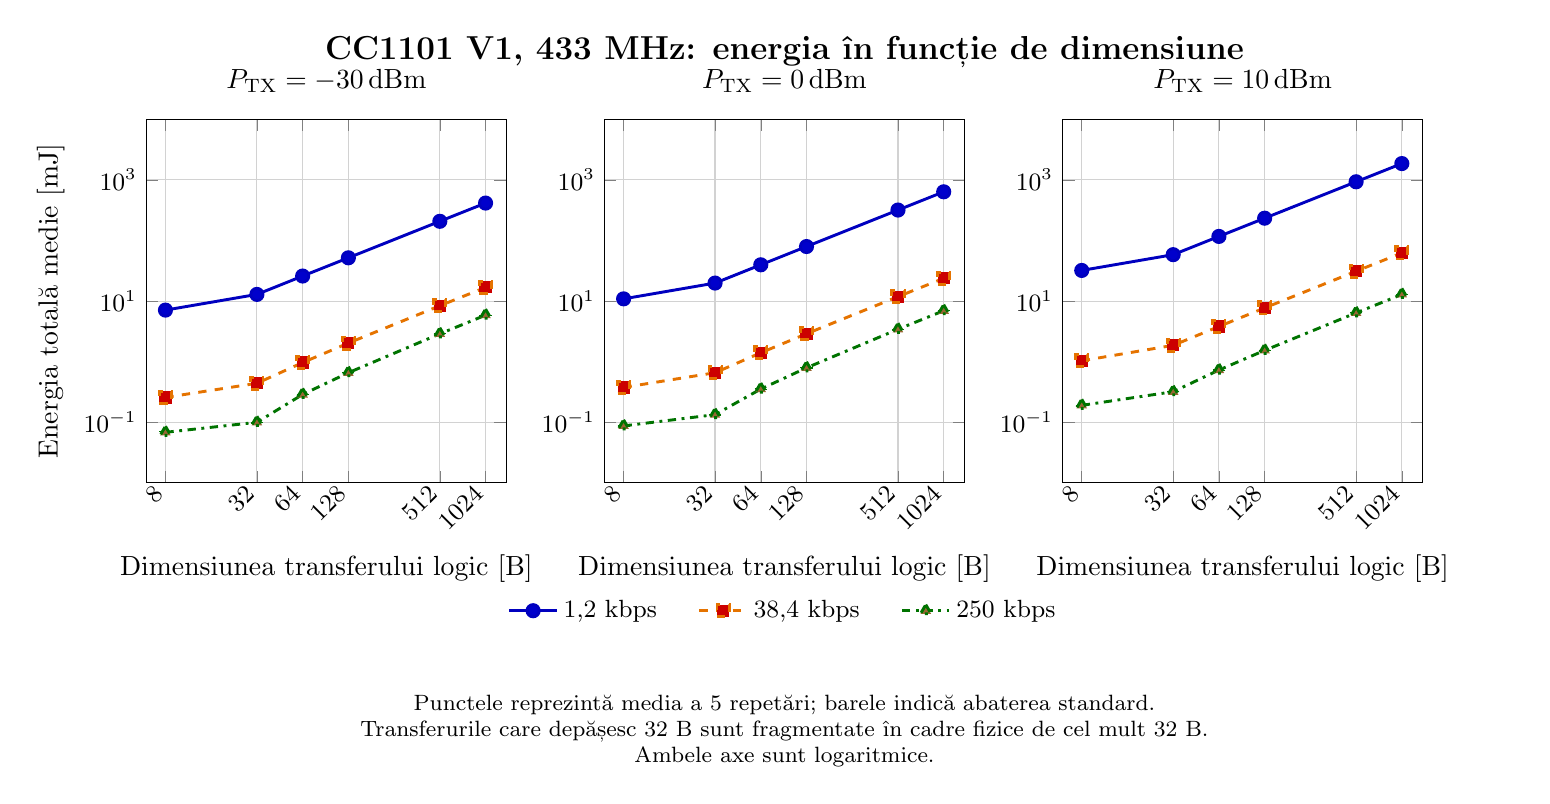
\begin{tikzpicture}
\begin{groupplot}[/pgf/number format/use comma,
  group style={group size=3 by 1, horizontal sep=1.25cm},
  width=6.15cm, height=6.2cm,
  xmode=log, log basis x={2},
  ymode=log, log basis y={10},
  ymin=0.01, ymax=10000,
  xmin=6, xmax=1400,
  xtick={8,32,64,128,512,1024},
  xticklabels={8,32,64,128,512,1024},
  x tick label style={rotate=45, anchor=east, font=\small},
  y tick label style={font=\small},
  grid=both, minor grid style={gray!15}, major grid style={gray!35},
  xlabel={Dimensiunea transferului logic [B]},
  every axis plot/.append style={line width=1.05pt},
  error bars/error bar style={line width=0.35pt},
  legend style={font=\small, draw=none, fill=none,
    at={(0.5,-0.29)}, anchor=north, legend columns=3,
    /tikz/every even column/.append style={column sep=0.45cm}},
]
\nextgroupplot[title={\(P_{\mathrm{TX}}=-30\,\mathrm{dBm}\)}, ylabel={Energia totală medie [mJ]}]
\addplot+[
  color=blue!75!black, solid, mark=*, mark size=2.2pt,
  error bars/.cd, y dir=both, y explicit,
] coordinates {
  (8,7.09843109) +- (0,0.0478225799)
  (32,12.888745) +- (0,0.0620221758)
  (64,25.895406) +- (0,0.0764140504)
  (128,51.7712326) +- (0,0.100162472)
  (512,207.182922) +- (0,0.213463707)
  (1024,414.088319) +- (0,0.181304985)
};
\addplot+[
  color=orange!90!black, dashed, mark=square*, mark size=2.2pt,
  error bars/.cd, y dir=both, y explicit,
] coordinates {
  (8,0.257303133) +- (0,0.00237886254)
  (32,0.440333595) +- (0,0.0011236768)
  (64,0.967497633) +- (0,0.00265361859)
  (128,2.02769133) +- (0,0.00336936332)
  (512,8.3719679) +- (0,0.00724980864)
  (1024,16.8276865) +- (0,0.0149853673)
};
\addplot+[
  color=green!45!black, dashdotted, mark=triangle*, mark size=2.2pt,
  error bars/.cd, y dir=both, y explicit,
] coordinates {
  (8,0.0683527131) +- (0,0.00107571668)
  (32,0.0999825356) +- (0,0.000585963609)
  (64,0.288035819) +- (0,0.00120425918)
  (128,0.657708845) +- (0,0.00215757994)
  (512,2.88415232) +- (0,0.00255903039)
  (1024,5.8576358) +- (0,0.00579388839)
};
\nextgroupplot[title={\(P_{\mathrm{TX}}=0\,\mathrm{dBm}\)}]
\addplot+[
  color=blue!75!black, solid, mark=*, mark size=2.2pt,
  error bars/.cd, y dir=both, y explicit,
] coordinates {
  (8,10.8881765) +- (0,0.00465029967)
  (32,19.8317351) +- (0,0.0602936922)
  (64,39.7009717) +- (0,0.049543019)
  (128,79.4944679) +- (0,0.125421507)
  (512,317.759631) +- (0,0.169732269)
  (1024,635.349066) +- (0,0.168979469)
};
\addlegendentry{1{,}2 kbps}
\addplot+[
  color=orange!90!black, dashed, mark=square*, mark size=2.2pt,
  error bars/.cd, y dir=both, y explicit,
] coordinates {
  (8,0.376161784) +- (0,0.00105469614)
  (32,0.657559199) +- (0,0.0018454898)
  (64,1.40215138) +- (0,0.0027499816)
  (128,2.89231373) +- (0,0.00189835199)
  (512,11.8347972) +- (0,0.00990021083)
  (1024,23.744598) +- (0,0.00906496518)
};
\addlegendentry{38{,}4 kbps}
\addplot+[
  color=green!45!black, dashdotted, mark=triangle*, mark size=2.2pt,
  error bars/.cd, y dir=both, y explicit,
] coordinates {
  (8,0.0872404574) +- (0,0.001581857)
  (32,0.133780291) +- (0,0.00177531691)
  (64,0.353770387) +- (0,0.0041071162)
  (128,0.792222769) +- (0,0.00397113332)
  (512,3.42693926) +- (0,0.00382138119)
  (1024,6.93115809) +- (0,0.00650667879)
};
\addlegendentry{250 kbps}
\nextgroupplot[title={\(P_{\mathrm{TX}}=10\,\mathrm{dBm}\)}]
\addplot+[
  color=blue!75!black, solid, mark=*, mark size=2.2pt,
  error bars/.cd, y dir=both, y explicit,
] coordinates {
  (8,32.0446747) +- (0,0.0370598432)
  (32,58.3144302) +- (0,0.0237579511)
  (64,116.672096) +- (0,0.111018904)
  (128,233.136856) +- (0,0.10288105)
  (512,930.375152) +- (0,0.301867613)
  (1024,1857.92992) +- (0,0.516739194)
};
\addplot+[
  color=orange!90!black, dashed, mark=square*, mark size=2.2pt,
  error bars/.cd, y dir=both, y explicit,
] coordinates {
  (8,1.03566357) +- (0,0.0033639912)
  (32,1.86283151) +- (0,0.00413811507)
  (64,3.81086863) +- (0,0.00510905198)
  (128,7.71433063) +- (0,0.00260353714)
  (512,31.0961076) +- (0,0.00925000582)
  (1024,62.2809748) +- (0,0.00981065808)
};
\addplot+[
  color=green!45!black, dashdotted, mark=triangle*, mark size=2.2pt,
  error bars/.cd, y dir=both, y explicit,
] coordinates {
  (8,0.190372885) +- (0,0.00139155929)
  (32,0.31967722) +- (0,0.00209535265)
  (64,0.729163421) +- (0,0.00128311596)
  (128,1.53636609) +- (0,0.00416778569)
  (512,6.38997669) +- (0,0.00765916982)
  (1024,12.8732147) +- (0,0.00806386669)
};
\end{groupplot}
\node[font=\bfseries\large] at ($(group c2r1.north)+(0,0.85cm)$)
  {CC1101 V1, 433 MHz: energia în funcție de dimensiune};
\node[font=\footnotesize, align=center, text width=18.5cm]
  at ($(group c2r1.south)+(0,-3.15cm)$)
  {Punctele reprezintă media a 5 repetări; barele indică abaterea standard.\\
   Transferurile care depășesc 32 B sunt fragmentate în cadre fizice de cel mult 32 B.\\
   Ambele axe sunt logaritmice.};
\end{tikzpicture}
\end{document}
